\section{Pattern Classification}
\label{sec:pattern-recognition}

In this section we have a closer look on pattern classification. The classification problem can be defined as follows: Given a $D$-dimensional input vector $x$ assign it to one of $C$ discrete classes. We refer to a given class by its number $c$ which lies in the range $1 \leq c \leq C$. The input vector $x$ is also called pattern or observation.

\subsection{Statistical Background}

Using a statistical approach we assume the pattern $x$ and the class $c$ to be random variables. Then $p(x)$ is the probability that we observe the pattern $x$ and $p(c)$ is the probability that we observe a pattern belonging to class $c$ \cite[p.~108-109]{Ney:1995}.

The classification task is to assign a pattern $x$ to its corresponding class. This can be accomplished by considering the class-conditional probability $p(c|x)$, that is the probability of pattern $x$ belonging to class $c$ \cite[p.~108-109]{Ney:1995}. By applying Bayes' theorem we can rewrite the class-conditional probability to give 
\begin{align}
p(c|x) = \frac{p(x|c) p(c)}{p(x)}\onedot
\end{align}
Then the class-conditional probability can be interpreted as posterior probability where $p(c)$ is the prior probability. The prior probability represents the probability of class $c$ before making an observation. The posterior probability describes the probability of class $c$ after observing the pattern $x$. \cite[p.~38-39]{Bishop:2006}.

\subsection{Bayes' Decision Rule}

Given the posterior probabilities $p(c|x)$ for all classes $c$ we can determine the class of $x$ using a decision rule. But we want to avoid decision errors. A decision error occurs if an observation vector $x$ is assigned to the wrong class. Bayes' decision rule given by
\begin{align}
c:\mathbb{R}^D \rightarrow \{1, \ldots, C\}, x \mapsto \underset{1 \leq c \leq C}{argmax} \left\{p(c | x)\right\}
\end{align}
results in a minimum number of decision errors \cite[p.~109]{Ney:1995}. But it assumes the true posterior probabilities to be known.

In practice the posterior probabilities $p(c|x)$ are unknown. Therefore, we may model the probability $p(c|x)$ directly (or indirectly by modeling $p(x | c)$ first) in the means of a so called model distribution $q_\theta(c|x)$ which depends on some parameters~$\theta$ \cite[p.~637-638]{Ney:2003}. Then we apply the model-based decision rule given by
\begin{align}
\label{eq:decision-rule}
c_\theta:\mathbb{R}^D \rightarrow \{1, \ldots, C\}, x \mapsto \underset{1 \leq c \leq C}{argmax} \left\{q_\theta(c | x)\right\}\onedot
\end{align}
Here we use the model distribution and, thus, the decision rule is fully dependent on the parameters $\theta$ \cite[p.~638]{Ney:2003}.

% In another approach we first model the class-conditional probabilities $p(x | c)$ using a model distribution $q_\theta (x | c)$. When assuming the prior distribution $p(c)$ to be known we can express the posterior probability by using  Bayes' theorem \cite[p.~337-638]{Ney:2003}:
%\begin{align}
%p(c | x) = \frac{q_\theta (x | c) p(c)}{p(x)} = \frac{q_\theta (x | c) p(c)}{\sum _{c = 1} ^C q_\theta (x | c) p(x)}\onedot
%\end{align}
% This approach is also known as generative model because by modeling $p(x | c)$ we are able to generate new patterns for each class \cite[p.~43]{Bishop:2006}.

\subsection{Maximum Likelihood Estimation}

Using a maximum likelihood approach we can estimate the unknown parameters of the model distribution. Therefore, we assume that the posterior probabilities are given by the model distribution $q_\theta(c | x)$ and the patterns $x_n$ are drawn independently from the distribution $q_\theta(c|x)$. We say the data points $x_n$ are independent and identically distributed \cite[p.~85-88]{DudaHartStork:2001}. Then the likelihood function is given by
\begin{align}
\mathcal{L}(\theta) = \prod _{n=1} ^N q_\theta(c_n | x_n)\onedot
\end{align}
where $c_n$ denotes the corresponding class of pattern $x_n$. We then want to maximize $\mathcal{L}(\theta)$. This is equivalent to minimizing the negative log-likelihood function which is given by
\begin{align}
- \log(\mathcal{L}(\theta)) = - \sum _{n=1} ^N \log(q_\theta(x_n | c))\onedot
\end{align}
Then, we can use the negative log-likelihood function as error function to train a neural network. The sum-of-squared error function and the cross-entropy error function can both be motivated using a maximum likelihood approach. We derive only the cross-entropy error function in the next section.

% \subsection{Binary Classification}
%
% As example we follow \cite[p.~234-235]{Bishop:2006} and consider binary classification. As in section \ref{sec:network-training} we assume a data set $T = \{(x_n, t_n) : 1 \leq n \leq N\}$ to be given where $t_n = c = 1$ refers to the first class whereas $t_n = c = 0$ refers to the second class.

% We model the posterior probability $p(c | x)$ in the means of a Bernoulli distribution
%\begin{align}
%q_\theta(c | x) = \theta^c (1 - \theta)^{1-c}
%\end{align}
% where $\theta$ is the probability of $x$ belonging to class $c = 1$. Then we have a single parameter~$\theta$. Now we can apply maximum likelihood estimation by assuming the training set to be a set of independent patterns $x_n$. Then, the likelihood function is given by
%\begin{align}
%\mathcal{L}(\theta) = \prod _{n = 1} ^N q_\theta(x_n | c) = \prod _{n = 1} ^N \theta ^{c_n} (1 - \theta)^{1 - c_n}\onedot
%\end{align}
%
% To derive an appropriate error function to train a neural network we consider the negative log-likelihood function:
%\begin{align}
%\label{eq:binary-classification-nloglikelihood}
%- \log(\mathcal{L}(\theta) & = - \sum _{n = 1} ^N \log\left(\theta ^{c_n} (1 - \theta)^{1 - c_n}\right)\notag\\
%& = - \sum _{n = 1} ^N c_n \log(\theta) + (1 - c_n) \log(1 - \theta) \onedot
%\end{align}
% We then consider the probability $\theta$ to be given by the network output. For this purpose we choose a sigmoidal activation function for the single output unit such that:
%\begin{align}
%y(x,w) = \frac{1}{1 + \exp(-z)} \in [0,1]
%\end{align}
% where $z$ is the actual input of the output unit as used in section \ref{sec:neural-networks}. By substituting $\theta = y(x,w)$ into equation \eqref{eq:binary-classification-nloglikelihood} we get the error function
%\begin{align}
%E(w) = - \sum _{n = 1} ^N c_n \log(y(x_n,w)) (1 - c_n) \log(1 - y(x_n,w))
%\end{align}
% which can be interpreted as a sepcial case of the cross-entropy error function introduced in section \ref{subsec:error-measures}.

\subsubsection{Derivation of Cross-Entropy}

We follow \cite[p.~232-236]{Bishop:2006} and consider the multiclass\footnote{Generally, we distinguish the binary classification problem in the case of $C = 2$ and the multiclass classification problem for $C > 2$.} classification problem. The target values $t_n$ follow the $1$--of--$C$ encoding scheme, that is the $i^\text{th}$ entry of $t_n$ equals $1$ iff the pattern $x_n$ belongs to class $i$.

We interpret the output of the neural network as the posterior probabilities
\begin{align}
p(c | x) = y_c(x,w)\onedot
\end{align}
The posterior probability for class $c$ can then be written as
\begin{align}
\label{eq:multiclass-posterior}
p(c | x) = \frac{p(x | c) p(c)}{\sum _{k = 1} ^C p(x | k) p(k)}\onedot
\end{align}
As output activation function we use the softmax function such that we can rewrite equation \eqref{eq:multiclass-posterior} to give
\begin{align}
p(c | x) = \frac{\exp({z_c})}{\sum _{k = 1} ^c \exp({z_k})} \text{ with } z_k = \log(p(k | x) p(k))\onedot
\end{align}
Here we model the posteriors in the means of the network output. This means that the parameters of the model distribution are given by the weights of the network. Given the probabilities $p(c | x)$ the maximum likelihood function takes the form
\begin{align}
\mathcal{L} (w) = \prod _{n = 1} ^N \prod _{c} ^C p(c | x_n)^{t_{nc}} =  \prod _{n = 1} ^N \prod _{c = 1} ^C y_c(x_n,w)^{t_{nc}}
\end{align}
and we can derive the error function $E(w)$ which is given by the cross-entropy error function already introduced in section \ref{subsec:error-measures}:
\begin{align}
E(w) = - \log(\mathcal{L}(w)) = - \sum _{n = 1} ^N \sum _{c = 1} ^C t_{nc} ln(y_c(w, x_n))\onedot
\end{align}
% In this case we directly modeled the posterior probabilities in the means of the network output. Thus the likelihood function estimates the parameters $w$ of the neural network rather than parameters for a model distribution.

\subsection{Application: Recognizing Handwritten Digits}

\begin{figure}
	\centering
	\subfigure[100 units, $\gamma = 0.5$]{
		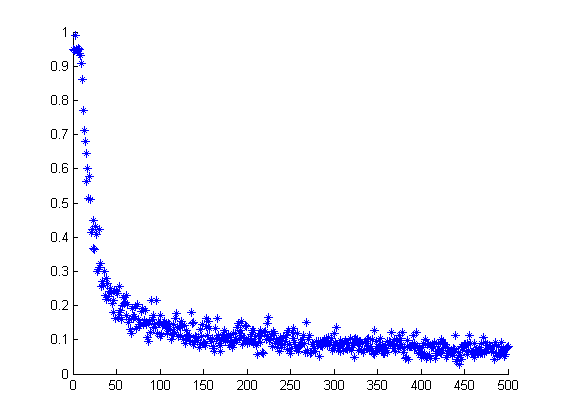
\includegraphics[width=0.2\textwidth]{images/100-500-0,5.png}
	}
	\subfigure[300 units, $\gamma = 0.5$]{
		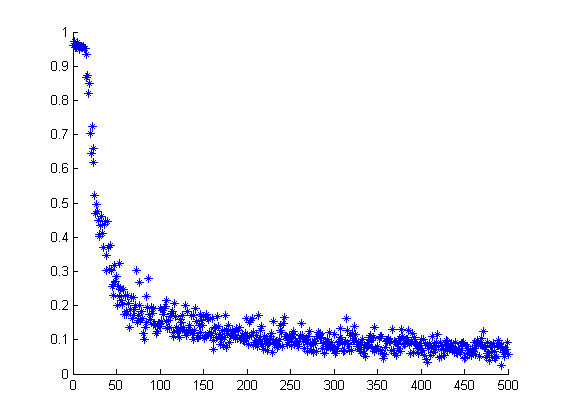
\includegraphics[width=0.2\textwidth]{images/100-500-0,5-300units.png}
	}
	\subfigure[400 units, $\gamma = 0.5$]{
		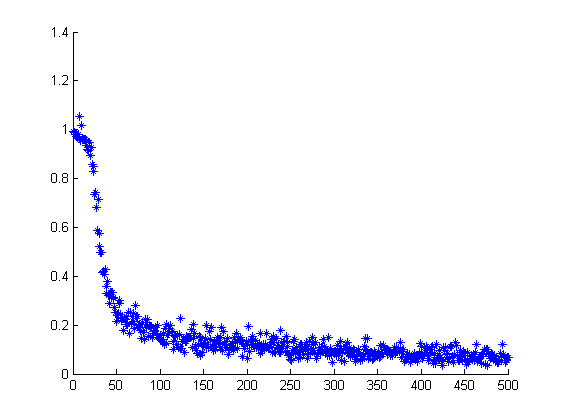
\includegraphics[width=0.2\textwidth]{images/100-500-0,5-400units.png}
	}
	\subfigure[500 units, $\gamma = 0.5$]{
		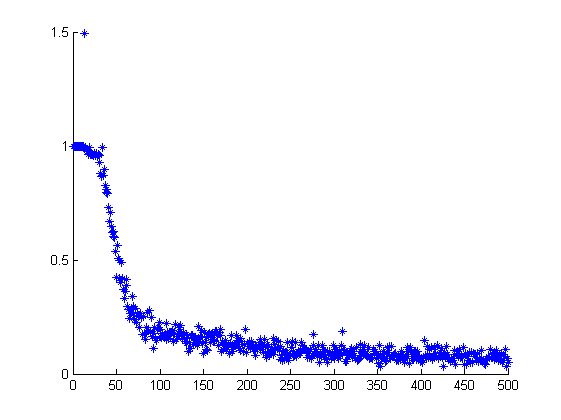
\includegraphics[width=0.2\textwidth]{images/100-500-0,5-500units.png}
	}
	\subfigure[600 units, $\gamma = 0.5$]{
		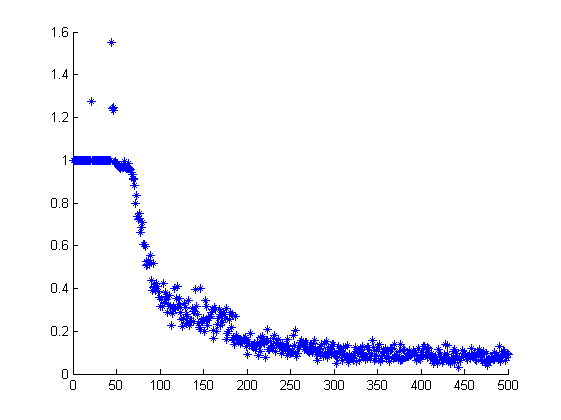
\includegraphics[width=0.2\textwidth]{images/100-500-0,5-600units.png}
	}
	\subfigure[700 units, $\gamma = 0.5$]{
		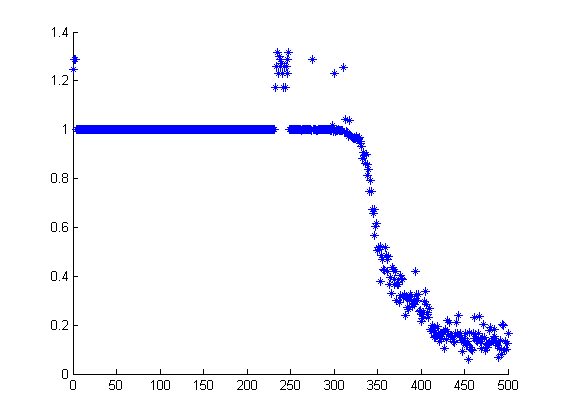
\includegraphics[width=0.2\textwidth]{images/100-500-0,5-700units.png}
	}
	\subfigure[750 units, $\gamma = 0.1$]{
		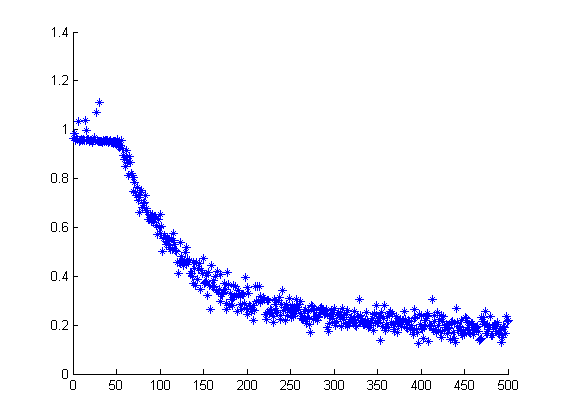
\includegraphics[width=0.2\textwidth]{images/100-500-0,1-750units.png}
	}
	\subfigure[800 units, $\gamma = 0.1$]{
		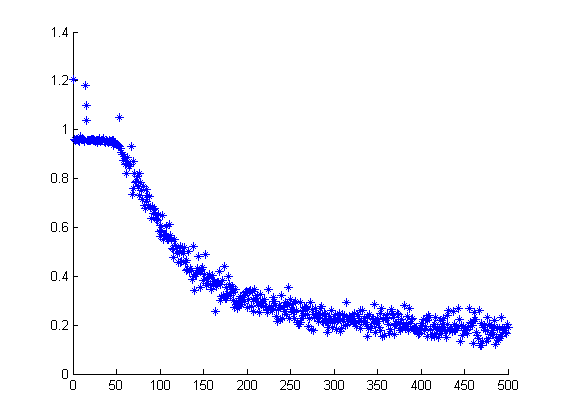
\includegraphics[width=0.2\textwidth]{images/100-500-0,1-800units.png}
	}
	\caption[Error on the training set during training.]{The error during training for different learning rates $\gamma$ and numbers of hidden units. The two-layer perceptron was trained with a batchsize of $100$ randomly chosen images iterated $500$ times. The error was measured using the sum-of-squared error function and plotted after each iteration.}
\end{figure}

Based on the MNIST dataset (available online at \href{http://yann.lecun.com/exdb/mnist/}{http://yann.lecun.com/exdb/mnist/}) we want to train a two-layer perceptron to recognize handwritten digits. The dataset provides a training set of $60,000$ images and a validation set of $10,000$ images. The images have $28 \times 28$ pixels of size and, thus, we may write an image as vector with $28 \cdot 28 = 784$ dimensions. The neural network will be trained using gradient descent for parameter optimization and the sum-of-squared error function. The training procedure is implemented in MatLab.

\subsubsection{Matrix Notation}

For implementing error backpropagation in MatLab it is convenient to introduce a matrix notation. We discuss the general case of a multilayer perceptron with $L$ layers. The output of all units in layer $l$ and their actual input can both be combined in vectors:
\begin{align}
y^{(l)} := \left( y_i ^{(l)} \right)_{i = 1}^{m^{(l)}} \text{ and } z^{(l)} := \left( z_i^{(l)} \right)_{i = 1}^{m^{(l)}}\onedot
\end{align}
When combining all weights $w_{ij}^{(l)}$ of layer $l$ in a single weight matrix we can express the propagation of an input vector through the network as several vector matrix products. The weight matrix $W^{(l)}$ is given by
\begin{align}
W^{(l)} := \left(w_{ij}^{(l)}\right)_{i,j = 1}^{m^{(l)},m^{(l-1)}}\onedot
\end{align}
Propagating the output vector of layer $(l - 1)$ denoted by $y^{(l-1)}$ through layer $l$ can then be written as
\begin{align}
y^{(l)} = f\left(W^{(l)}y^{(l-1)}\right)
\end{align}
where $f$ operates element by element. Given the error vector $\delta ^{(l+1)}$ defined as
\begin{align}
\delta^{(l+1)} := \left(\delta_i^{(l+1)}\right)_{i = 1}^{m^{(l+1)}}
\end{align}
for layer $(l+1)$ we can use the transpose of the weight matrix to give
\begin{align}
\delta ^{(l)} = f'(z^{(l)}) \bullet \left(W^{(l)}\right)^{tr} \delta^{(l+1)}
\end{align}
where $f'$ operates element by element and $\bullet$ denotes the component-wise multiplication.

\subsubsection{Implementation and Results}

The MNIST dataset is provided in the IDX file format. To get the images as vector with $784$ dimensions we use two functions \lstinline{loadMNISTImages} and \lstinline{loadMNISTLabels} which can be found online at \href{http://ufldl.stanford.edu/}{http://ufldl.stanford.edu/}.

Appendix \ref{lst:train-two-layer-perceptron} shows the implementation of the training procedure. The activation function and its derivative are passed as parameters. We use the logistic sigmoid, which is shown in appendix \ref{lst:activation-function}, as activation function for both the hidden and the output layer. The number of hidden units and the learning rate are adjustable. The weight matrices for both layers are initialized randomly and normalized afterwards (lines 29 to 35). We apply stochastic training in so called epochs, that is for each epoch we train the network on randomly selected input values (lines 42 to 61). The number of randomly selected input values to use for training is defined by the parameter \lstinline{batchSize}. After each epoch we plot the current error on the same input values as the network was trained on (lines 63 to 73).

For comparing different configurations we use the validation set. The validation procedure, which counts the number of correctly classified images, is shown in appendix \ref{lst:validation}. The accuracy is measured as the quotient of correctly classified images and the total number of images. Figure \ref{fig:results} shows some of the results.

\begin{figure}[t!]
	\centering
	\subfigure[$500$ epochs with batch size $100$.]{
		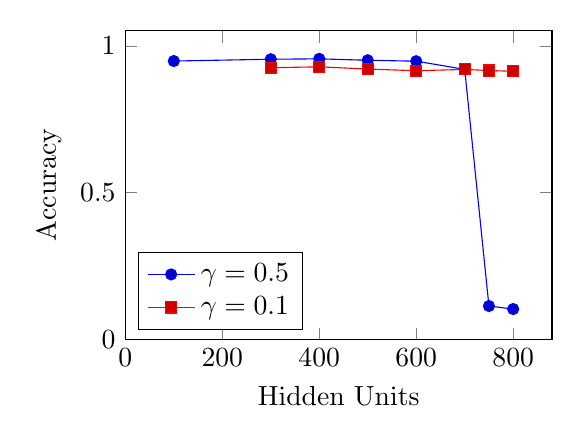
\begin{tikzpicture}
			\begin{axis}[height=5.5cm,width=7cm,ylabel=Accuracy,xlabel=Hidden Units,xmin=0,ymin=0,legend pos=south west]
				\addplot+[blue] coordinates{(100,1-0.0519)(300,1-0.0457)(400,1-0.0444)(500,1-0.0492)(600,1-0.0524)(700,1-0.0801)(750,1-0.8865)(800,1-0.8968)};
				\addlegendentry{$\gamma = 0.5$}
				\addplot+[red] coordinates{(300,1-0.0747)(400,1-0.0716)(500,1-0.0791)(600,1-0.0849)(700,1-0.0804)(750,1-0.0842)(800,1-0.0868)};
				\addlegendentry{$\gamma = 0.1$}
			\end{axis}
		\end{tikzpicture}
		\label{subfig:results-units}
	}
	\subfigure[$500$ epochs with learning rate $\gamma = 0.5$.]{
		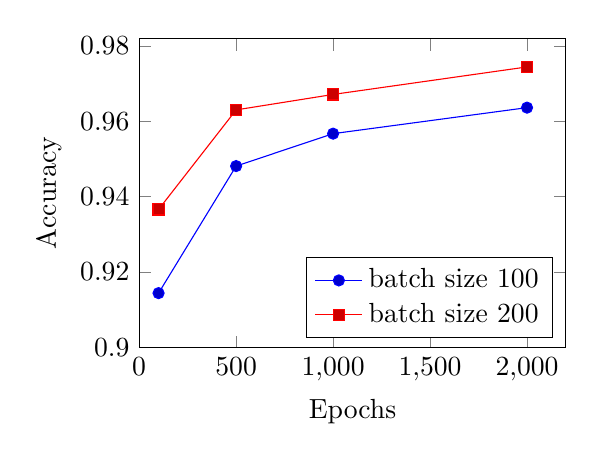
\begin{tikzpicture}
			\begin{axis}[height=5.5cm,width=7cm,ylabel=Accuracy,xlabel=Epochs,xmin=0,ymin=0.9,legend pos=south east]
				\addplot+[blue] coordinates{(100,1-0.0856)(500,1-0.0519)(1000,1-0.0433)(2000,1-0.0364)};
				\addlegendentry{batch size 100}
				\addplot+[red] coordinates{(100,1-0.0634)(500,1-0.0370)(1000,1-0.0329)(2000,1-0.0256)};
				\addlegendentry{batch size 200}
			\end{axis}
		\end{tikzpicture}
		\label{subfig:results-epochs}
	}
	\caption[Results of training a two-layer perceptron using the MNIST dataset.]{Figure \ref{subfig:results-units} plots the achieved accuracy depending on the number of hidden units for a fixed learning rate $\gamma = 0.5$. For $750$ or more units we need to adjust the learning rate in order to ensure convergence. But this may result in slow convergence such that we get worse results for few hidden units. Figure \ref{subfig:results-epochs} shows the impact of increasing the number of epochs. As we would expect, the accuracy increases with rising training set.}
	\label{fig:results}
\end{figure}
